\documentclass[17pt,a4paper,landscape]{extarticle}
\usepackage[margin=2.35cm,top=0.12cm,left=1.05cm]{geometry}
\usepackage{amsmath}
\usepackage{amssymb}
\usepackage{tasks}
\usepackage{tikz}
\usepackage{xcolor}
\usepackage[sfdefault,lf]{FiraSans}
\renewcommand{\familydefault}{\sfdefault}
\setlength{\parindent}{0pt}
\pagestyle{empty}
\settasks{label=\textbf{\arabic*.}, label-width=2.2em, item-indent=2.95em, column-sep=2.1cm, after-item-skip=4.7em}
\renewcommand{\arraystretch}{1.15}
\everymath{\displaystyle}

\begin{document}
\sffamily
\boldmath

\boldmath

\boldmath

\boldmath

\boldmath

\boldmath

{\LARGE \textbf{Volume of cubes and cuboids — Proficient}}
\begin{tasks}(3)
\task Find the volume of this cuboid.\\[0.4em]
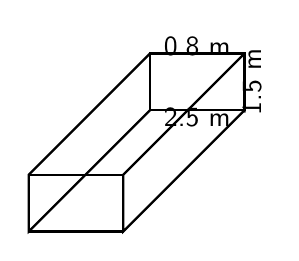
\begin{tikzpicture}[x=0.12cm,y=0.12cm,baseline=(current bounding box.center)]
  \draw[thick] (0,0,0) -- (10,0,0) -- (10,6,0) -- (0,6,0) -- cycle;
  \draw[thick] (0,0,0) -- (0,0,4) -- (0,6,4) -- (0,6,0);
  \draw[thick] (10,0,0) -- (10,0,4) -- (10,6,4) -- (10,6,0);
  \draw[thick] (0,0,4) -- (10,0,4) -- (10,6,4) -- (0,6,4) -- cycle;
  \draw[dashed] (0,0,0) -- (0,0,4);
  \draw[dashed] (10,0,0) -- (10,0,4);
  \draw[dashed] (0,6,0) -- (0,6,4);
  \draw[dashed] (10,6,0) -- (10,6,4);
  \node at (5,-0.8) {2.5 m};
  \node[rotate=90] at (10.8,3) {1.5 m};
  \node at (5,6.8) {0.8 m};
\end{tikzpicture}
\task Find the volume of this cube.\\[0.4em]
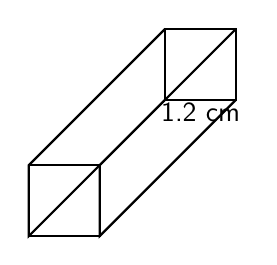
\begin{tikzpicture}[x=0.2cm,y=0.2cm,baseline=(current bounding box.center)]
  \draw[thick] (0,0,0) -- (4.5,0,0) -- (4.5,4.5,0) -- (0,4.5,0) -- cycle;
  \draw[thick] (0,0,0) -- (0,0,4.5) -- (0,4.5,4.5) -- (0,4.5,0);
  \draw[thick] (4.5,0,0) -- (4.5,0,4.5) -- (4.5,4.5,4.5) -- (4.5,4.5,0);
  \draw[thick] (0,0,4.5) -- (4.5,0,4.5) -- (4.5,4.5,4.5) -- (0,4.5,4.5) -- cycle;
  \draw[dashed] (0,0,0) -- (0,0,4.5);
  \draw[dashed] (4.5,0,0) -- (4.5,0,4.5);
  \draw[dashed] (0,4.5,0) -- (0,4.5,4.5);
  \draw[dashed] (4.5,4.5,0) -- (4.5,4.5,4.5);
  \node at (2.25,-0.8) {1.2 cm};
\end{tikzpicture}
\task A storage box is 80 cm long, 50 cm wide, and 40 cm high. What is its volume in cubic centimetres? In cubic metres?
\task A cube has volume 125 cm\mbox{$^3$}. What is its side length?
\task A cuboid has volume 240 mm\mbox{$^3$}, width 6 mm, and height 5 mm. What is its length?
\task How many 1 cm cubes would fit inside a 1 m cube?
\task Convert 2.5 m\mbox{$^3$} to cm\mbox{$^3$}.
\task Convert 7500 mm\mbox{$^3$} to cm\mbox{$^3$}.
\task A fish tank is 60 cm long, 30 cm wide, and 40 cm high. What is its volume in litres? (1 litre = 1000 cm\mbox{$^3$})
\task A cube has side length 0.3 m. What is its volume in cm\mbox{$^3$}?
\task A cuboid has dimensions 2.4 m by 1.8 m by 0.9 m. What is its volume in m\mbox{$^3$} and cm\mbox{$^3$}?
\task A box has volume 1.2 m\mbox{$^3$}. If its length is 2 m and width is 0.6 m, what is its height?
\task Which has greater volume: a cube with side 8 cm or a cuboid 10 cm × 7 cm × 4 cm?
\task A room is 5 m long, 4 m wide, and 2.5 m high. What is its volume?
\task A cube and a cuboid have the same volume. The cube has side 6 cm. The cuboid has length 9 cm and width 4 cm. What is the height of the cuboid?
\task Explain why 1 m\mbox{$^3$} = 1,000,000 cm\mbox{$^3$}.
\task A shipping container is 12 m long, 2.4 m wide, and 2.6 m high. What is its volume?
\end{tasks}

\end{document}